%DO NOT MESS AROUND WITH THE CODE ON THIS PAGE UNLESS YOU %REALLY KNOW WHAT YOU ARE DOING
\chapter*{Experimental Research}
\addcontentsline{toc}{chapter}{Experimental Research}

\section*{ Rectangular Pulse } 
\addcontentsline{toc}{section}{Rectangular Pulse }
 
\begin{figure}[H]
\centering
{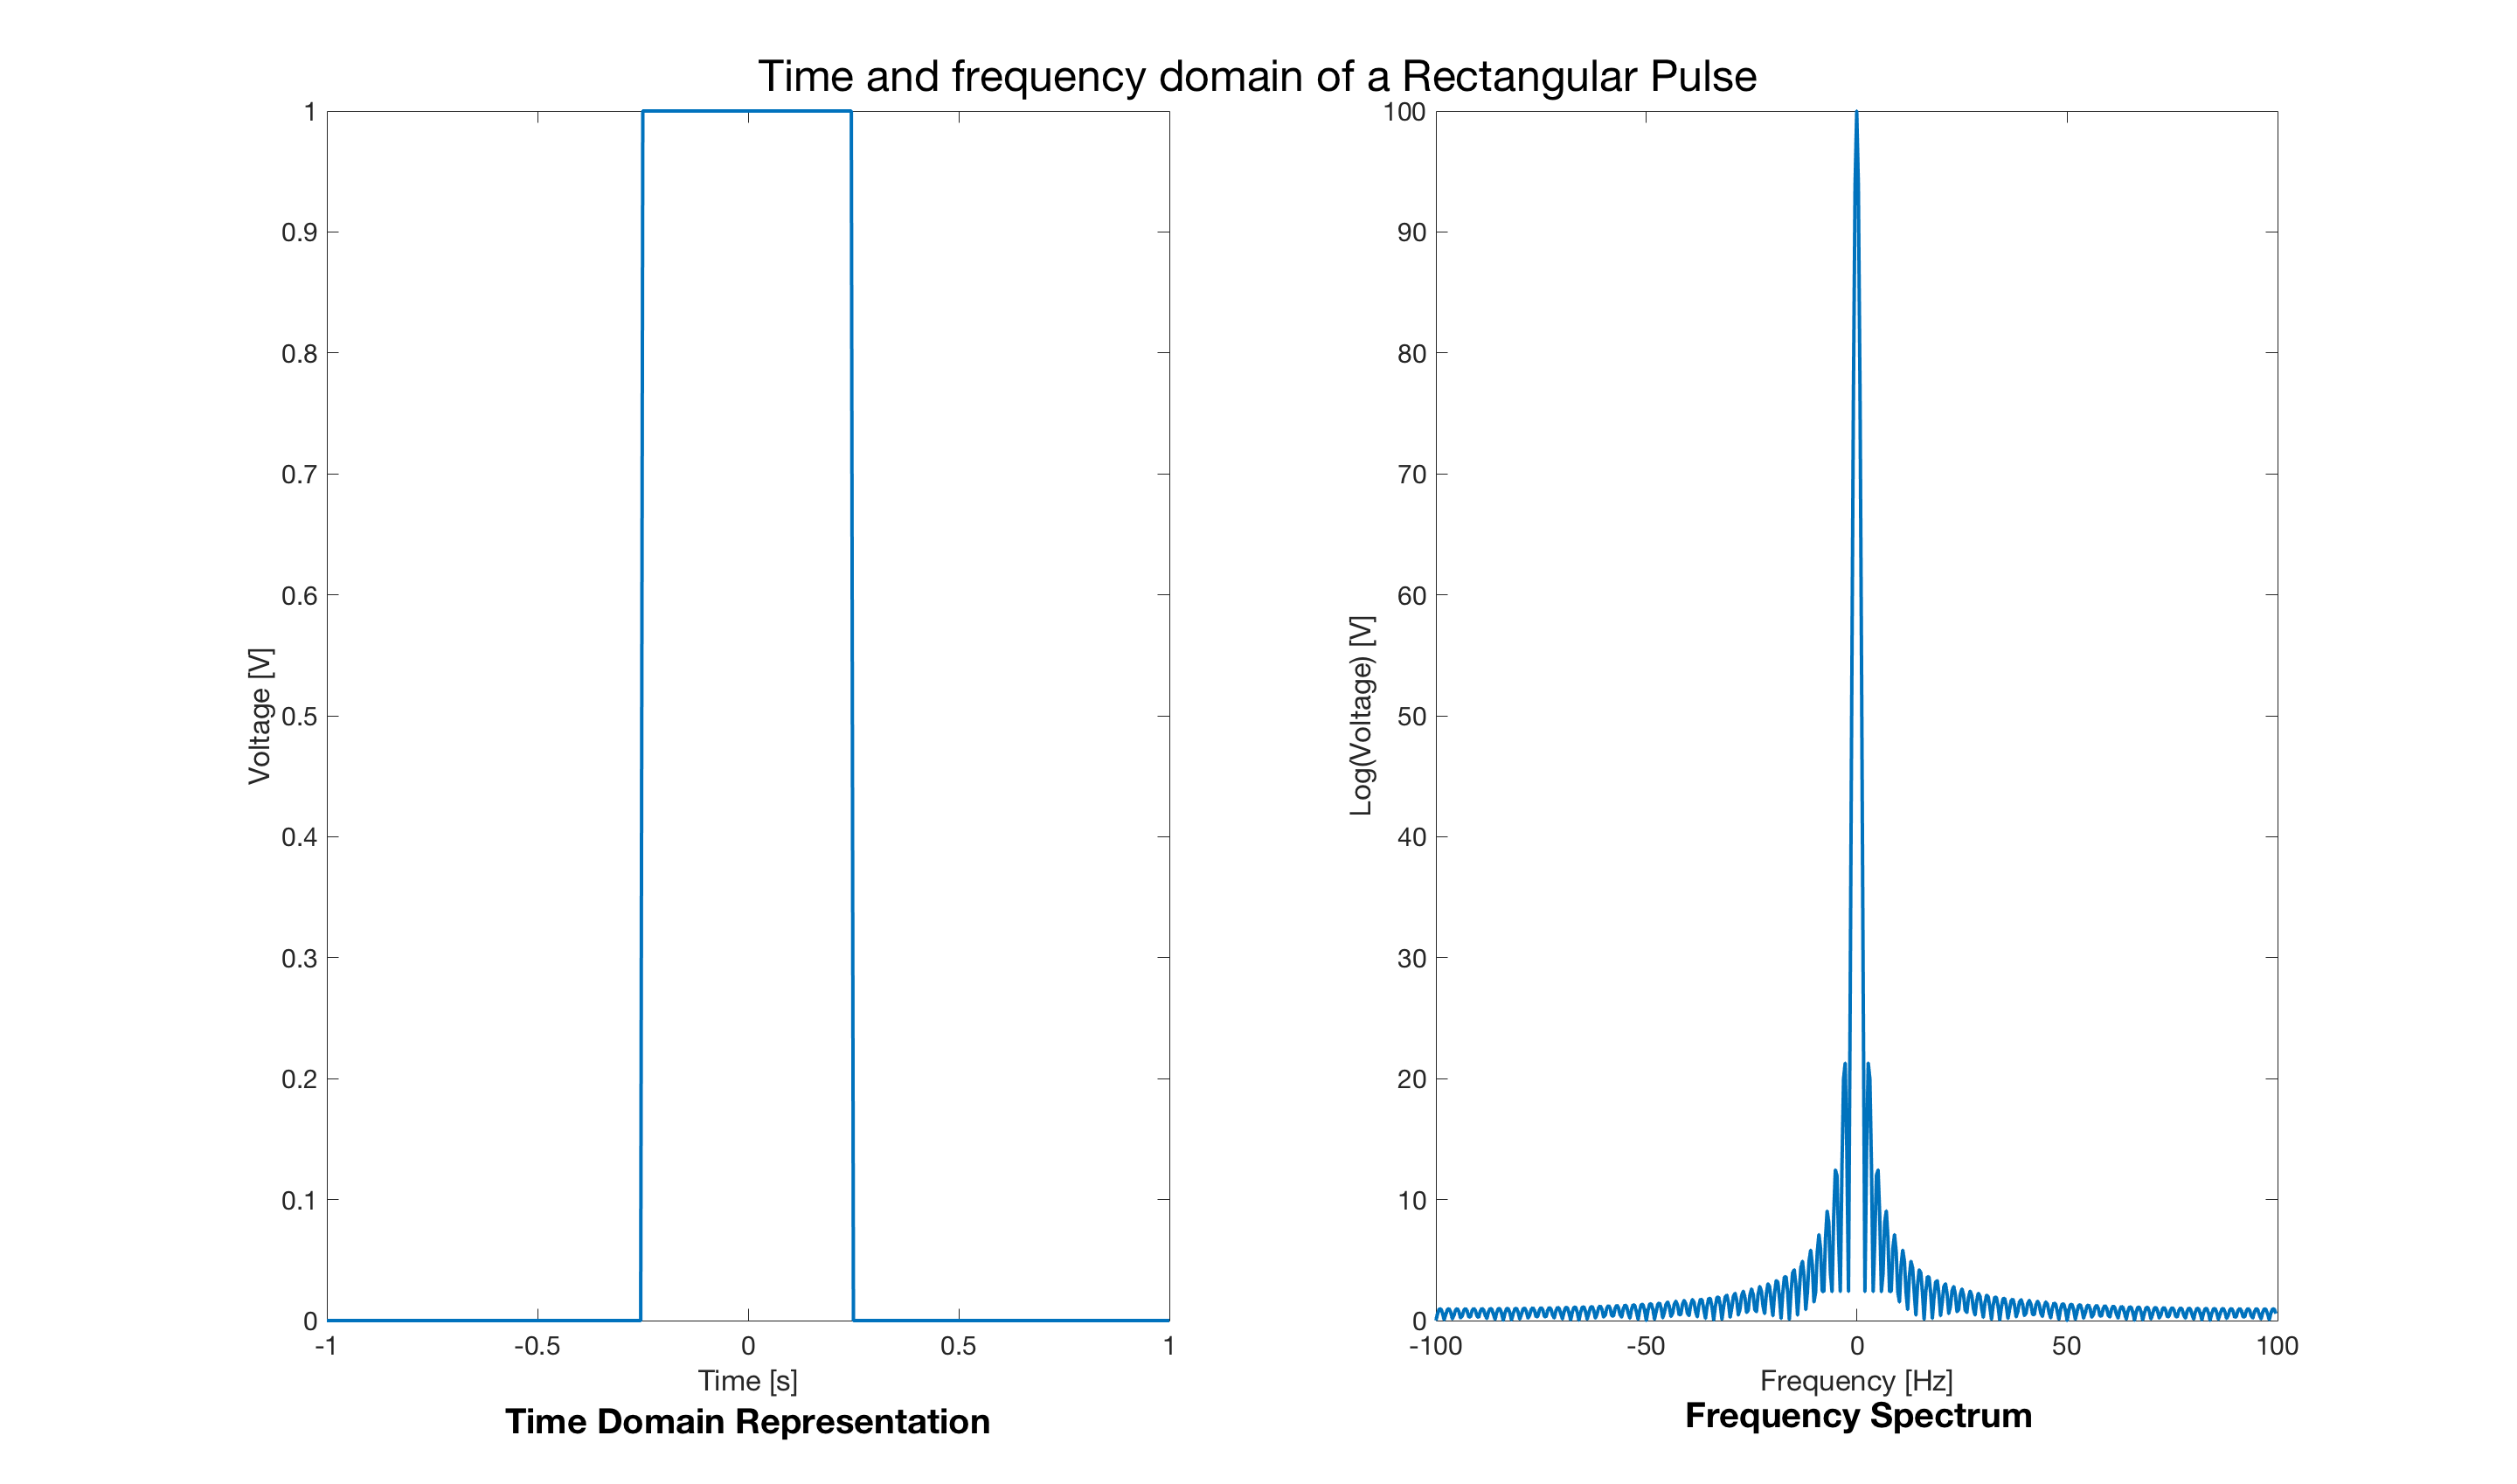
\includegraphics[scale=0.18]{usp8_1.png}}
\caption{ A rectangular pulse in time domain (left) along with its spectrum (right)}
\end{figure}

\begin{figure}[H]
\centering
{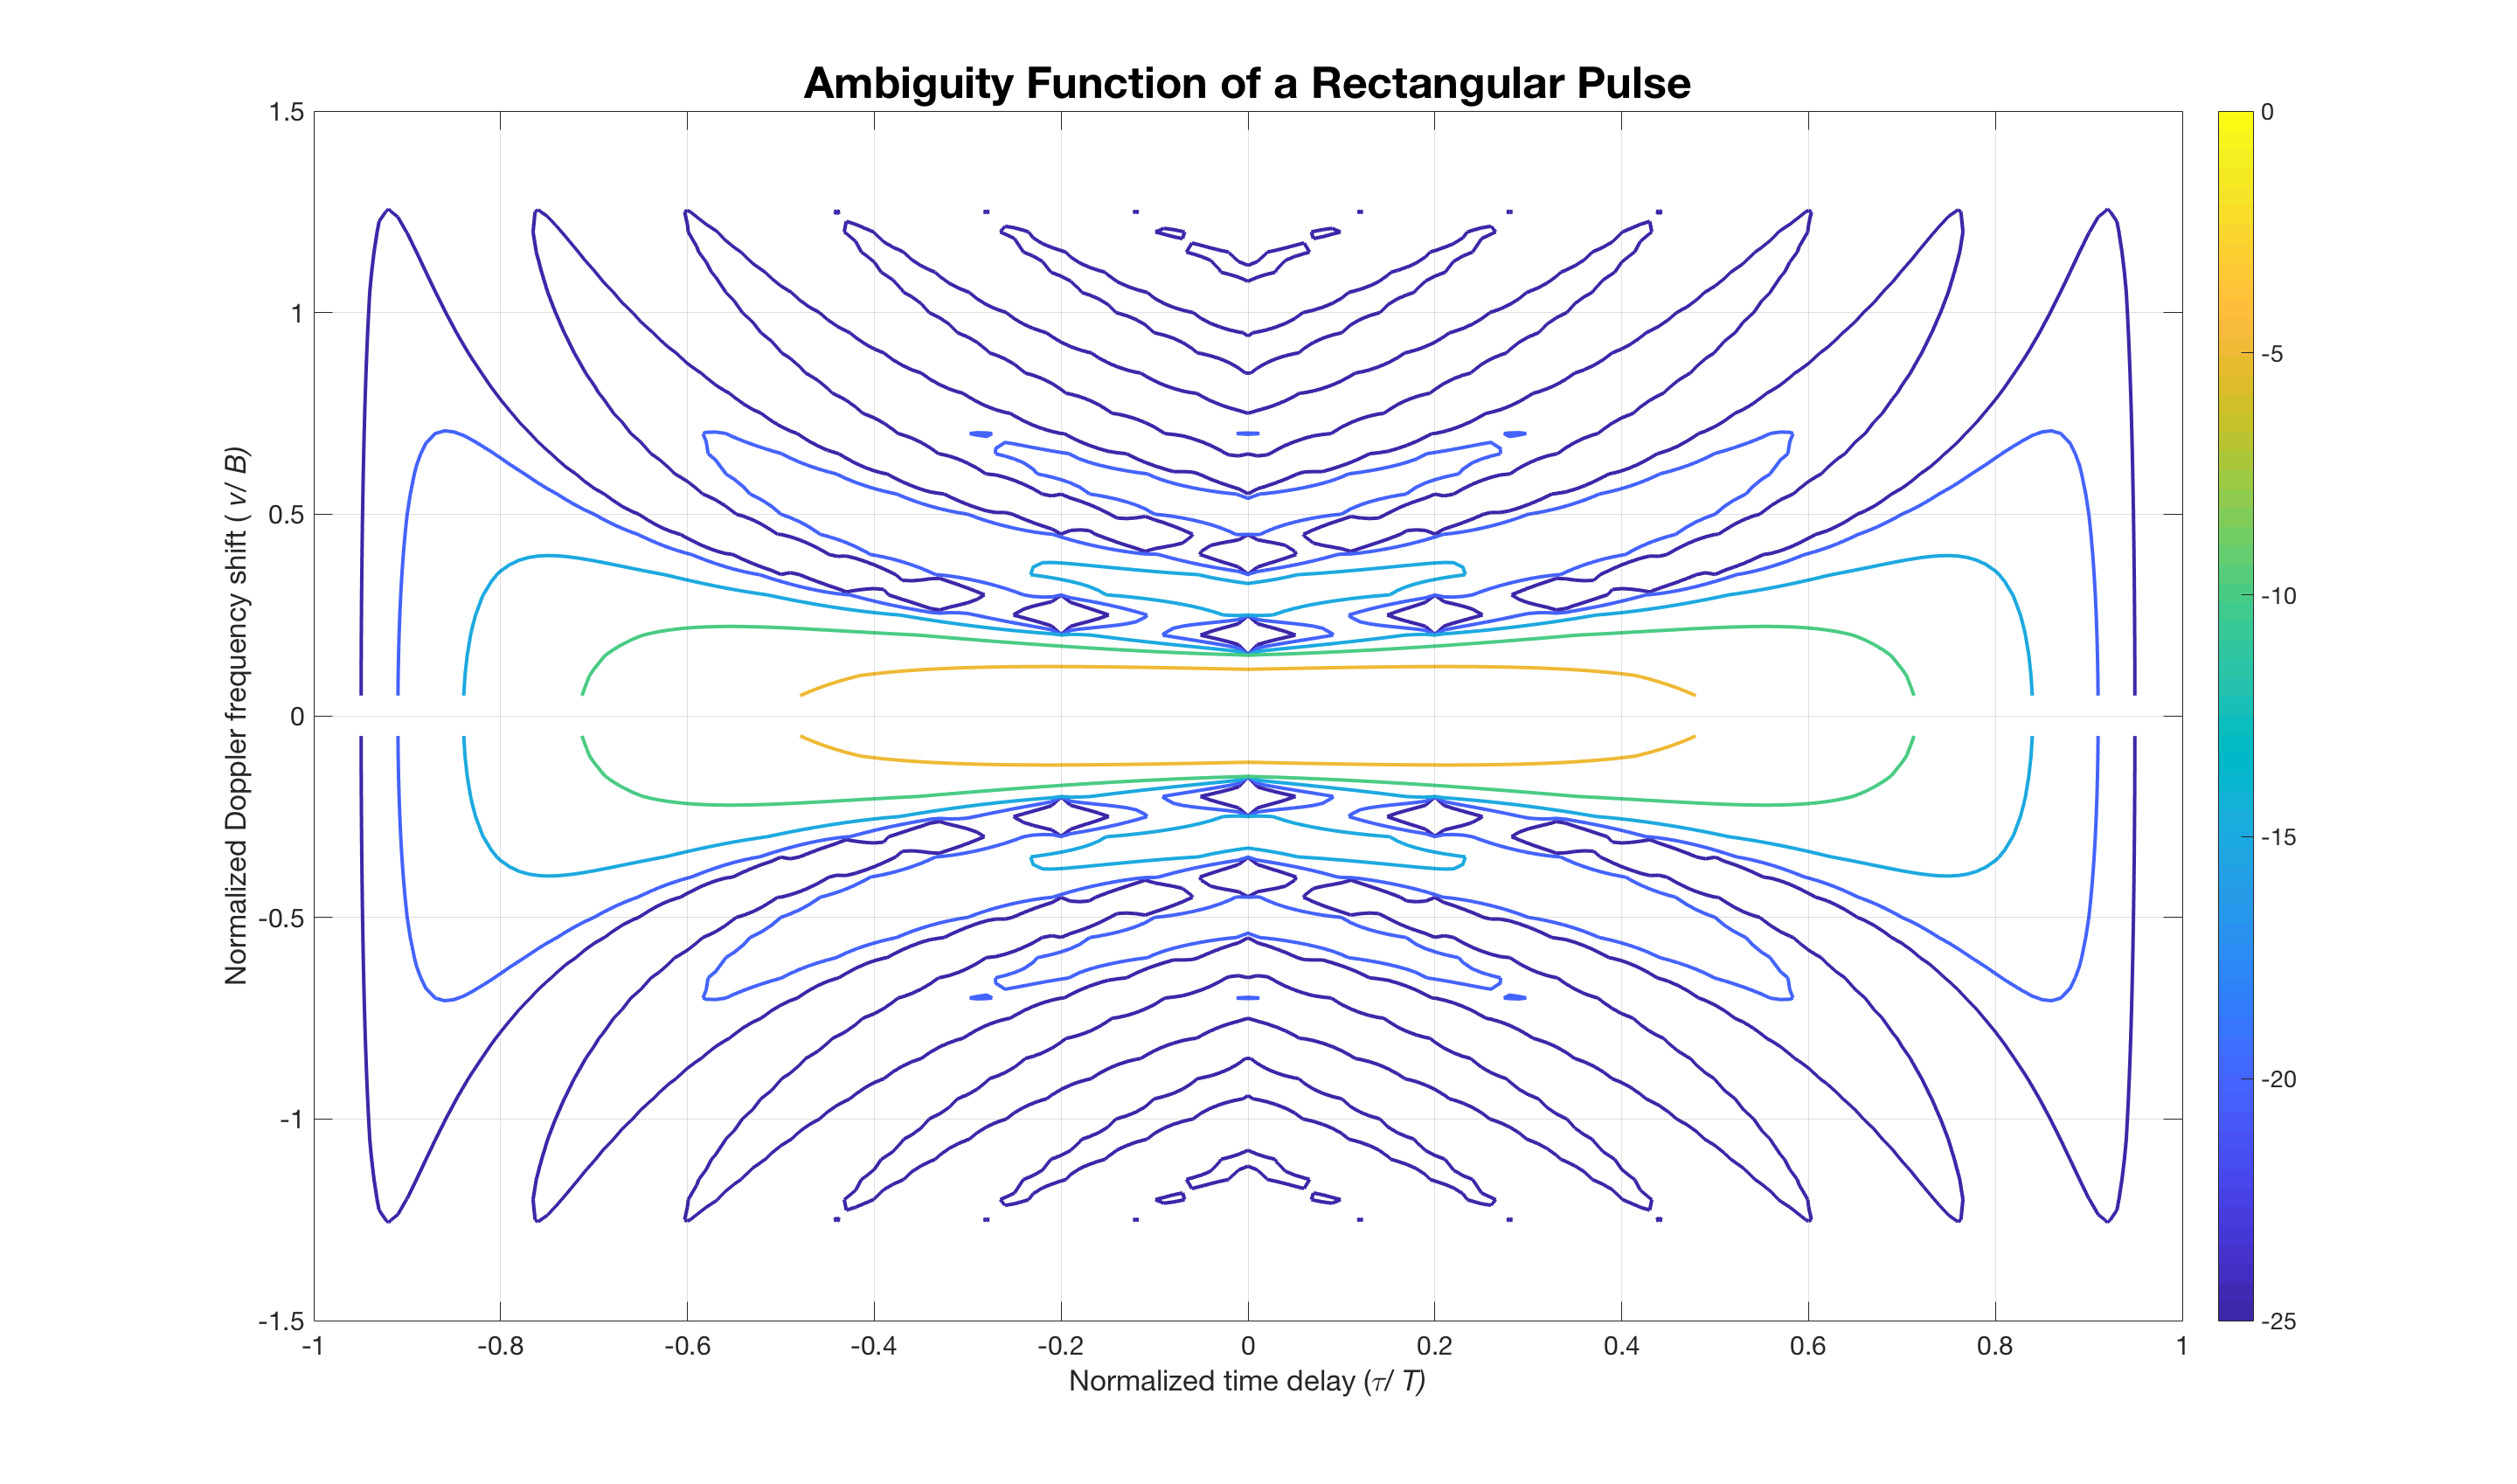
\includegraphics[scale=0.18]{usp8_4.png}}
\caption{ Ambiguity function of a rectangular pulse }
\end{figure}

\newpage
\section*{ Linear Frequency Modulated pulse with a Rectangular Envelope }
\addcontentsline{toc}{section}{Linear Frequency Modulated pulse with a Rectangular Envelope }

\begin{figure}[H]
\centering
{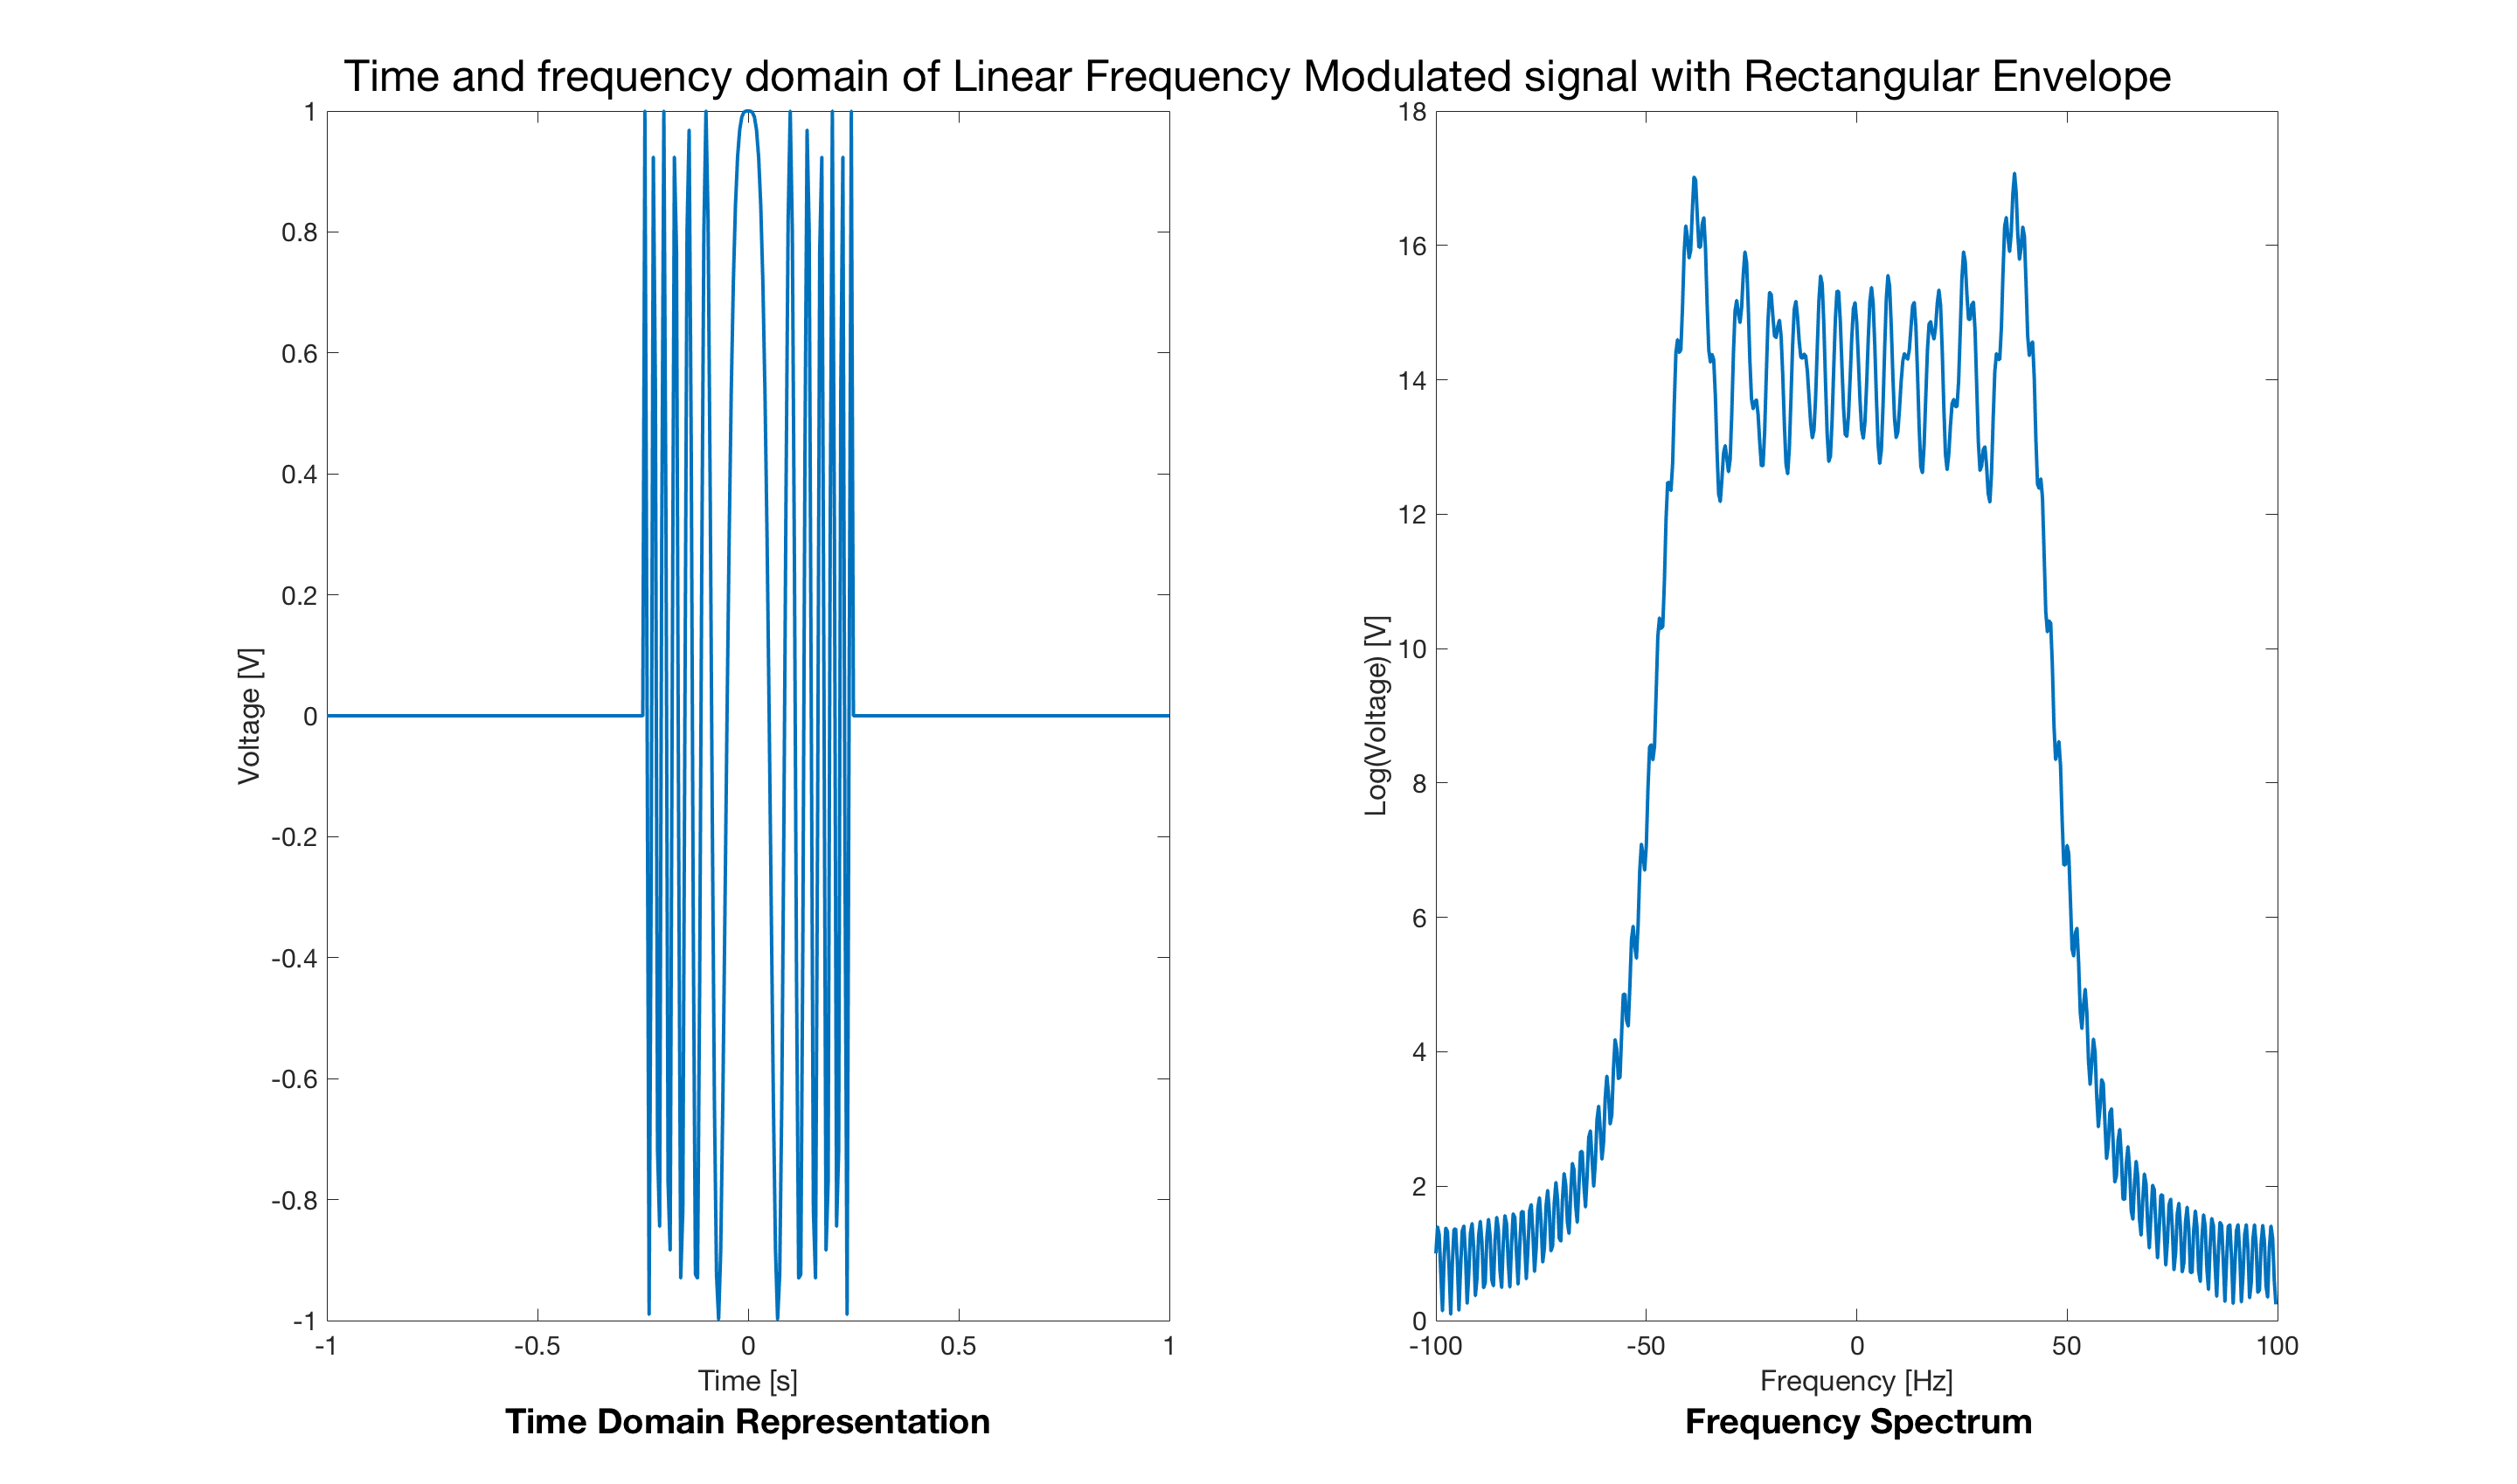
\includegraphics[scale=0.18]{usp8_2.png}}
\caption{ A Linear Frequency Modulated (LFM) pulse with rectangular envelope in time domain (left) along with its spectrum (right)}
\end{figure}

\begin{figure}[H]
\centering
{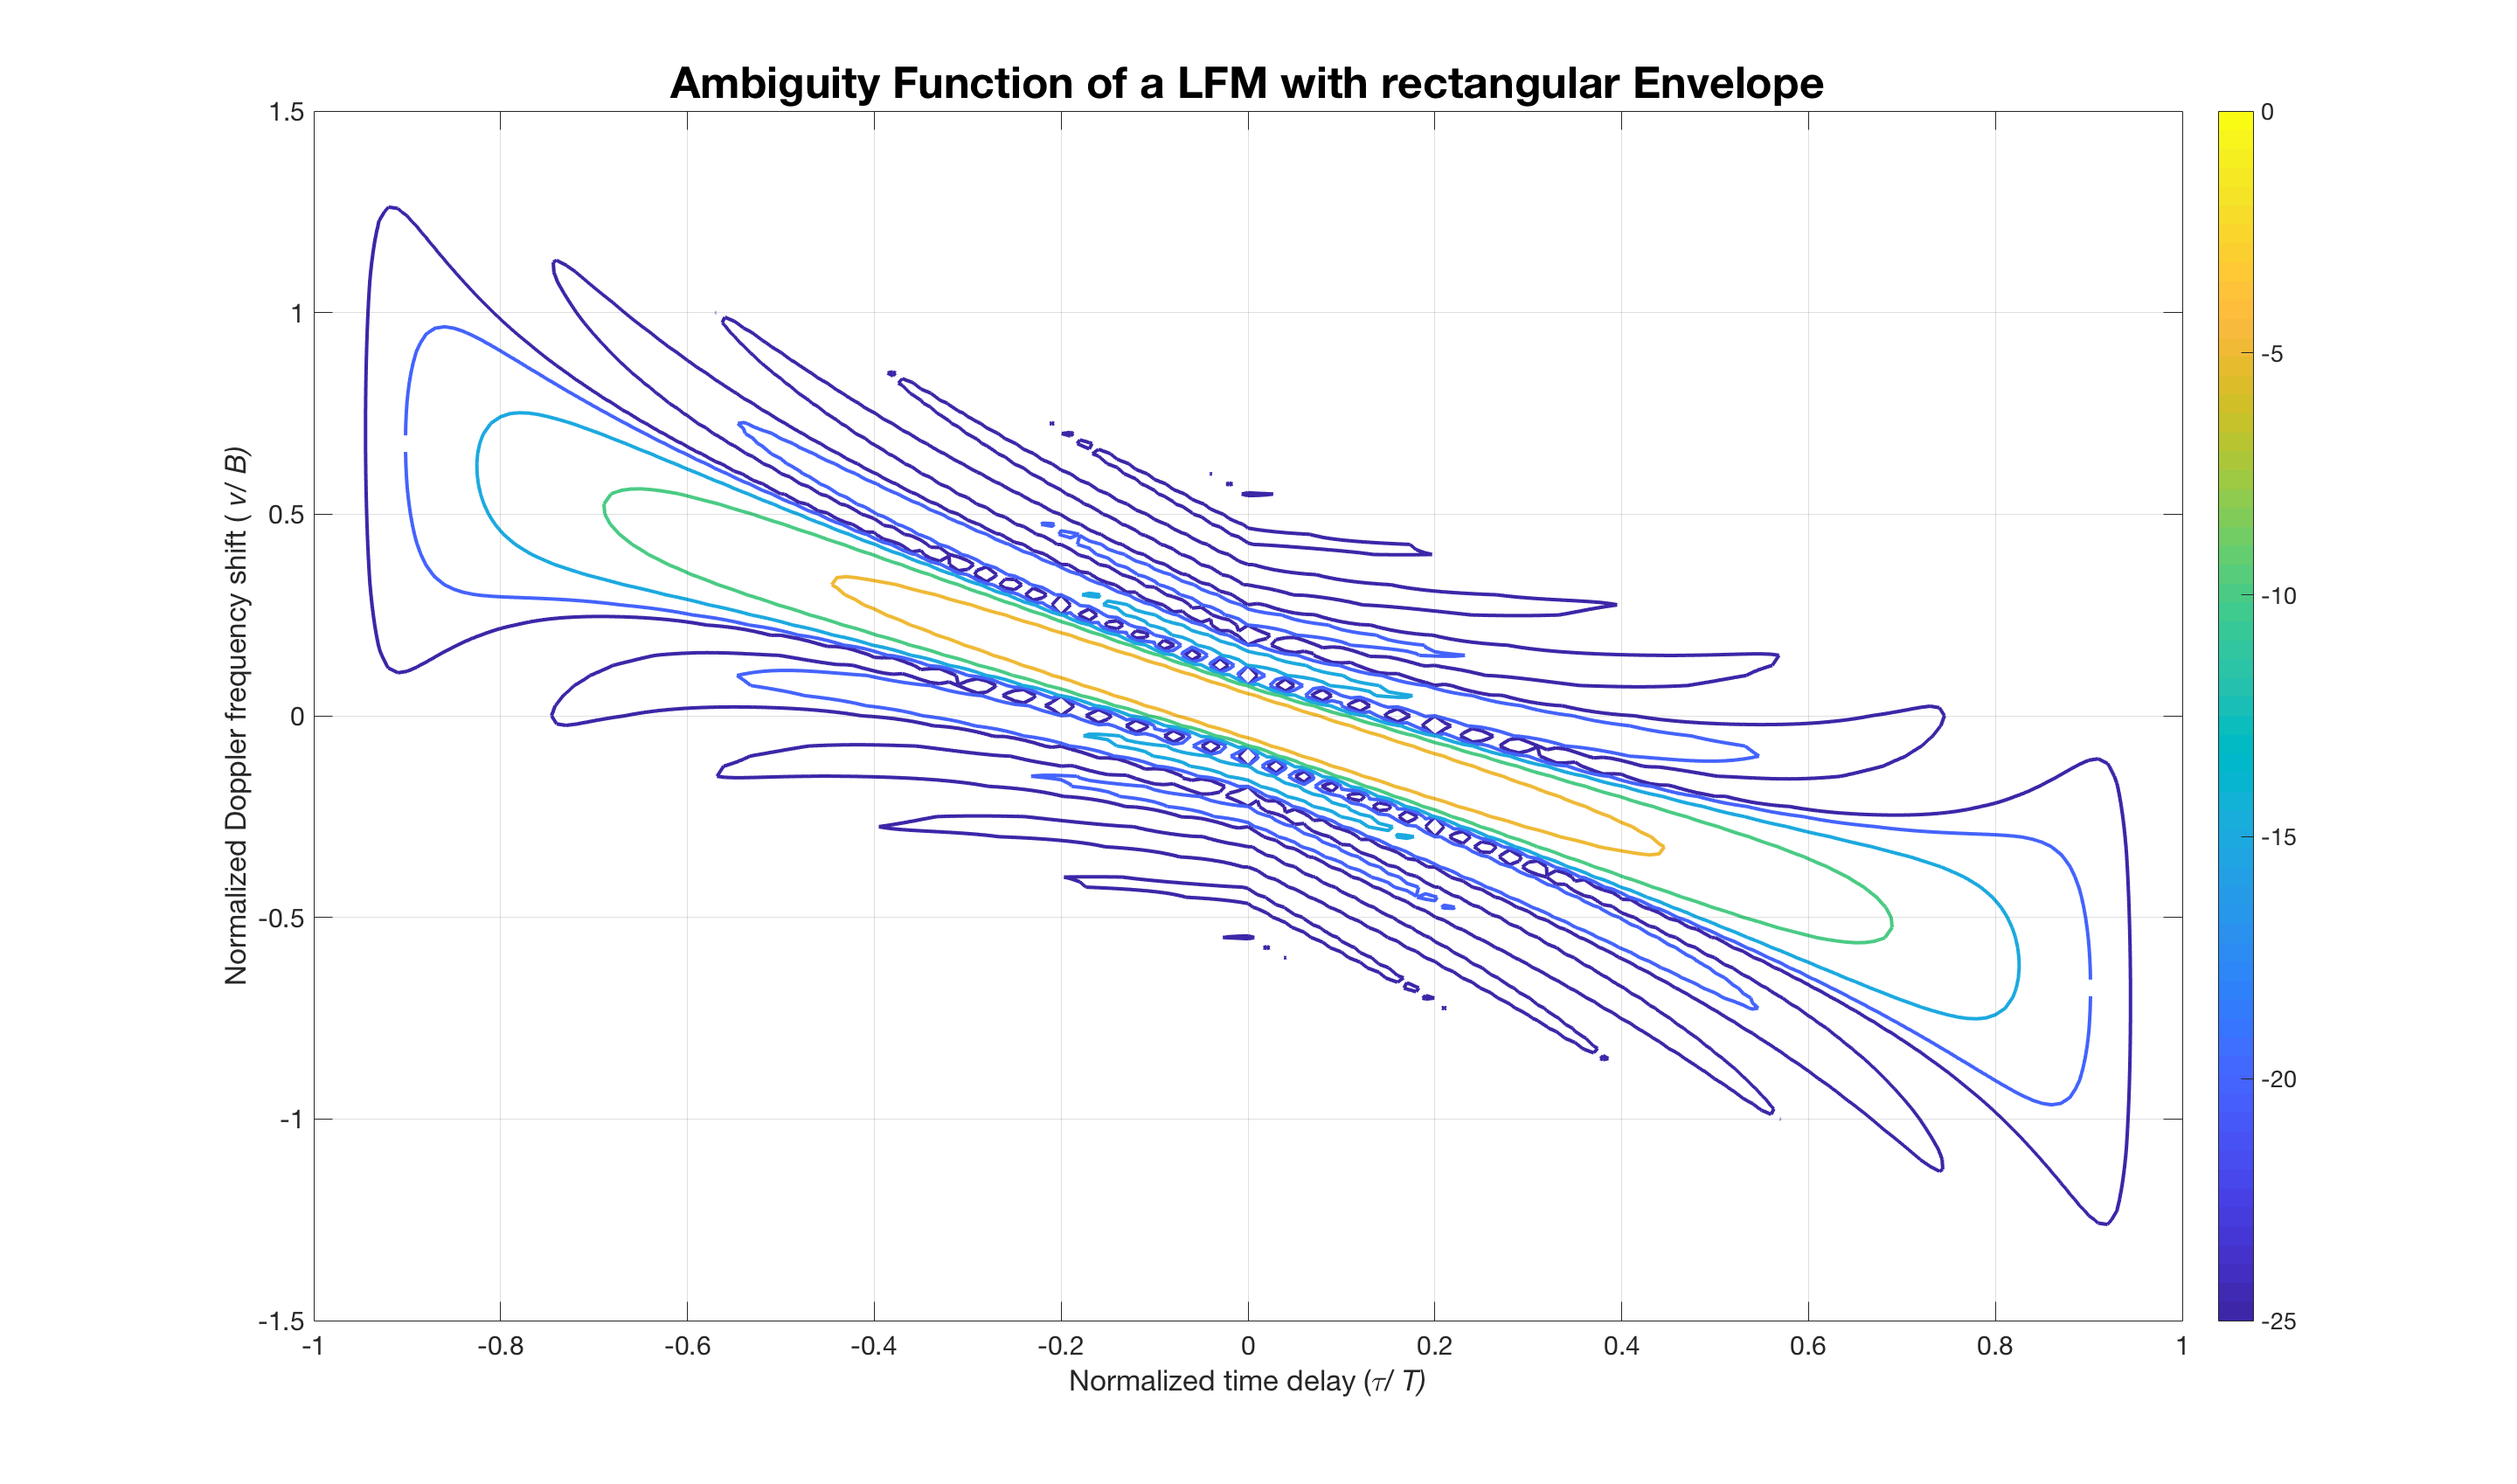
\includegraphics[scale=0.18]{usp8_5.png}}
\caption{ The ambiguity function of a Linear Frequency Modulated (LFM) pulse with rectangular envelope }
\end{figure}

\newpage

\section*{Linear Frequency Modulated pulse with a Gaussian Envelope } 
\addcontentsline{toc}{section}{Linear Frequency Modulated pulse with a Gaussian Envelope }

\begin{figure}[H]
\centering
{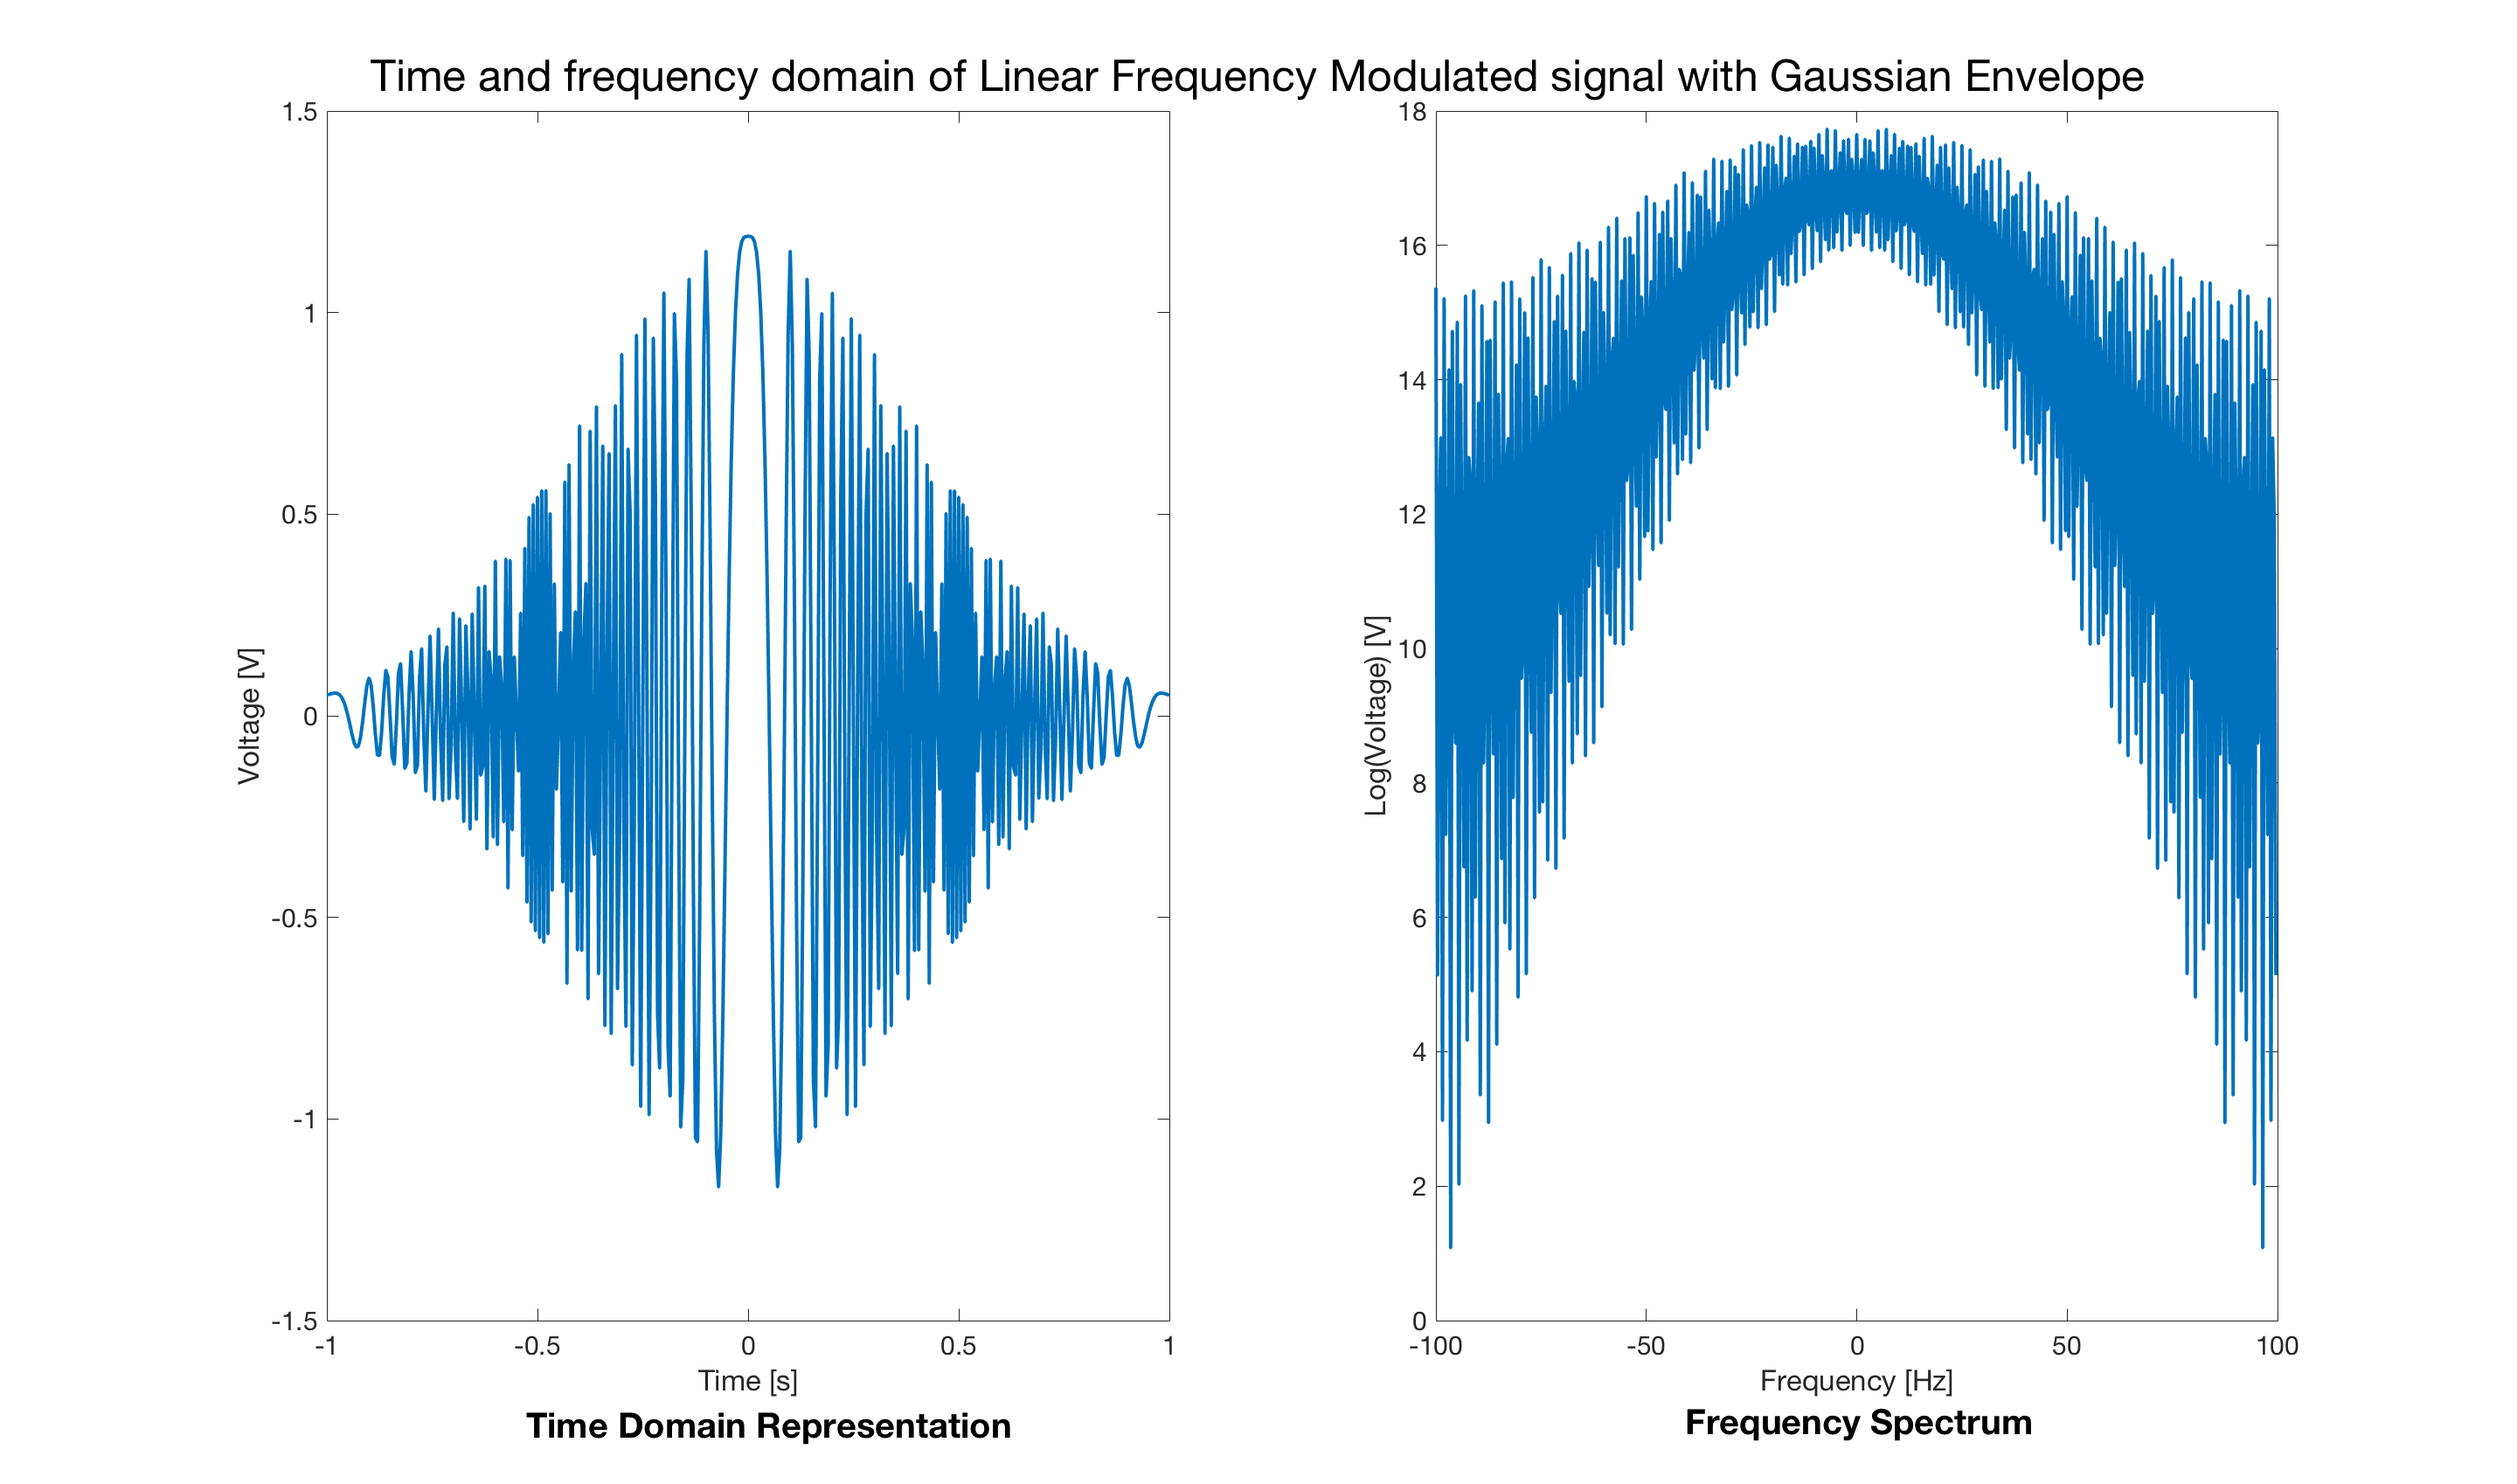
\includegraphics[scale=0.18]{usp8_3.png}}
\caption{ A Linear Frequency Modulated (LFM) pulse with Gaussian envelope in time domain (left) along with its spectrum (right)}
\end{figure}

\begin{figure}[H]
\centering
{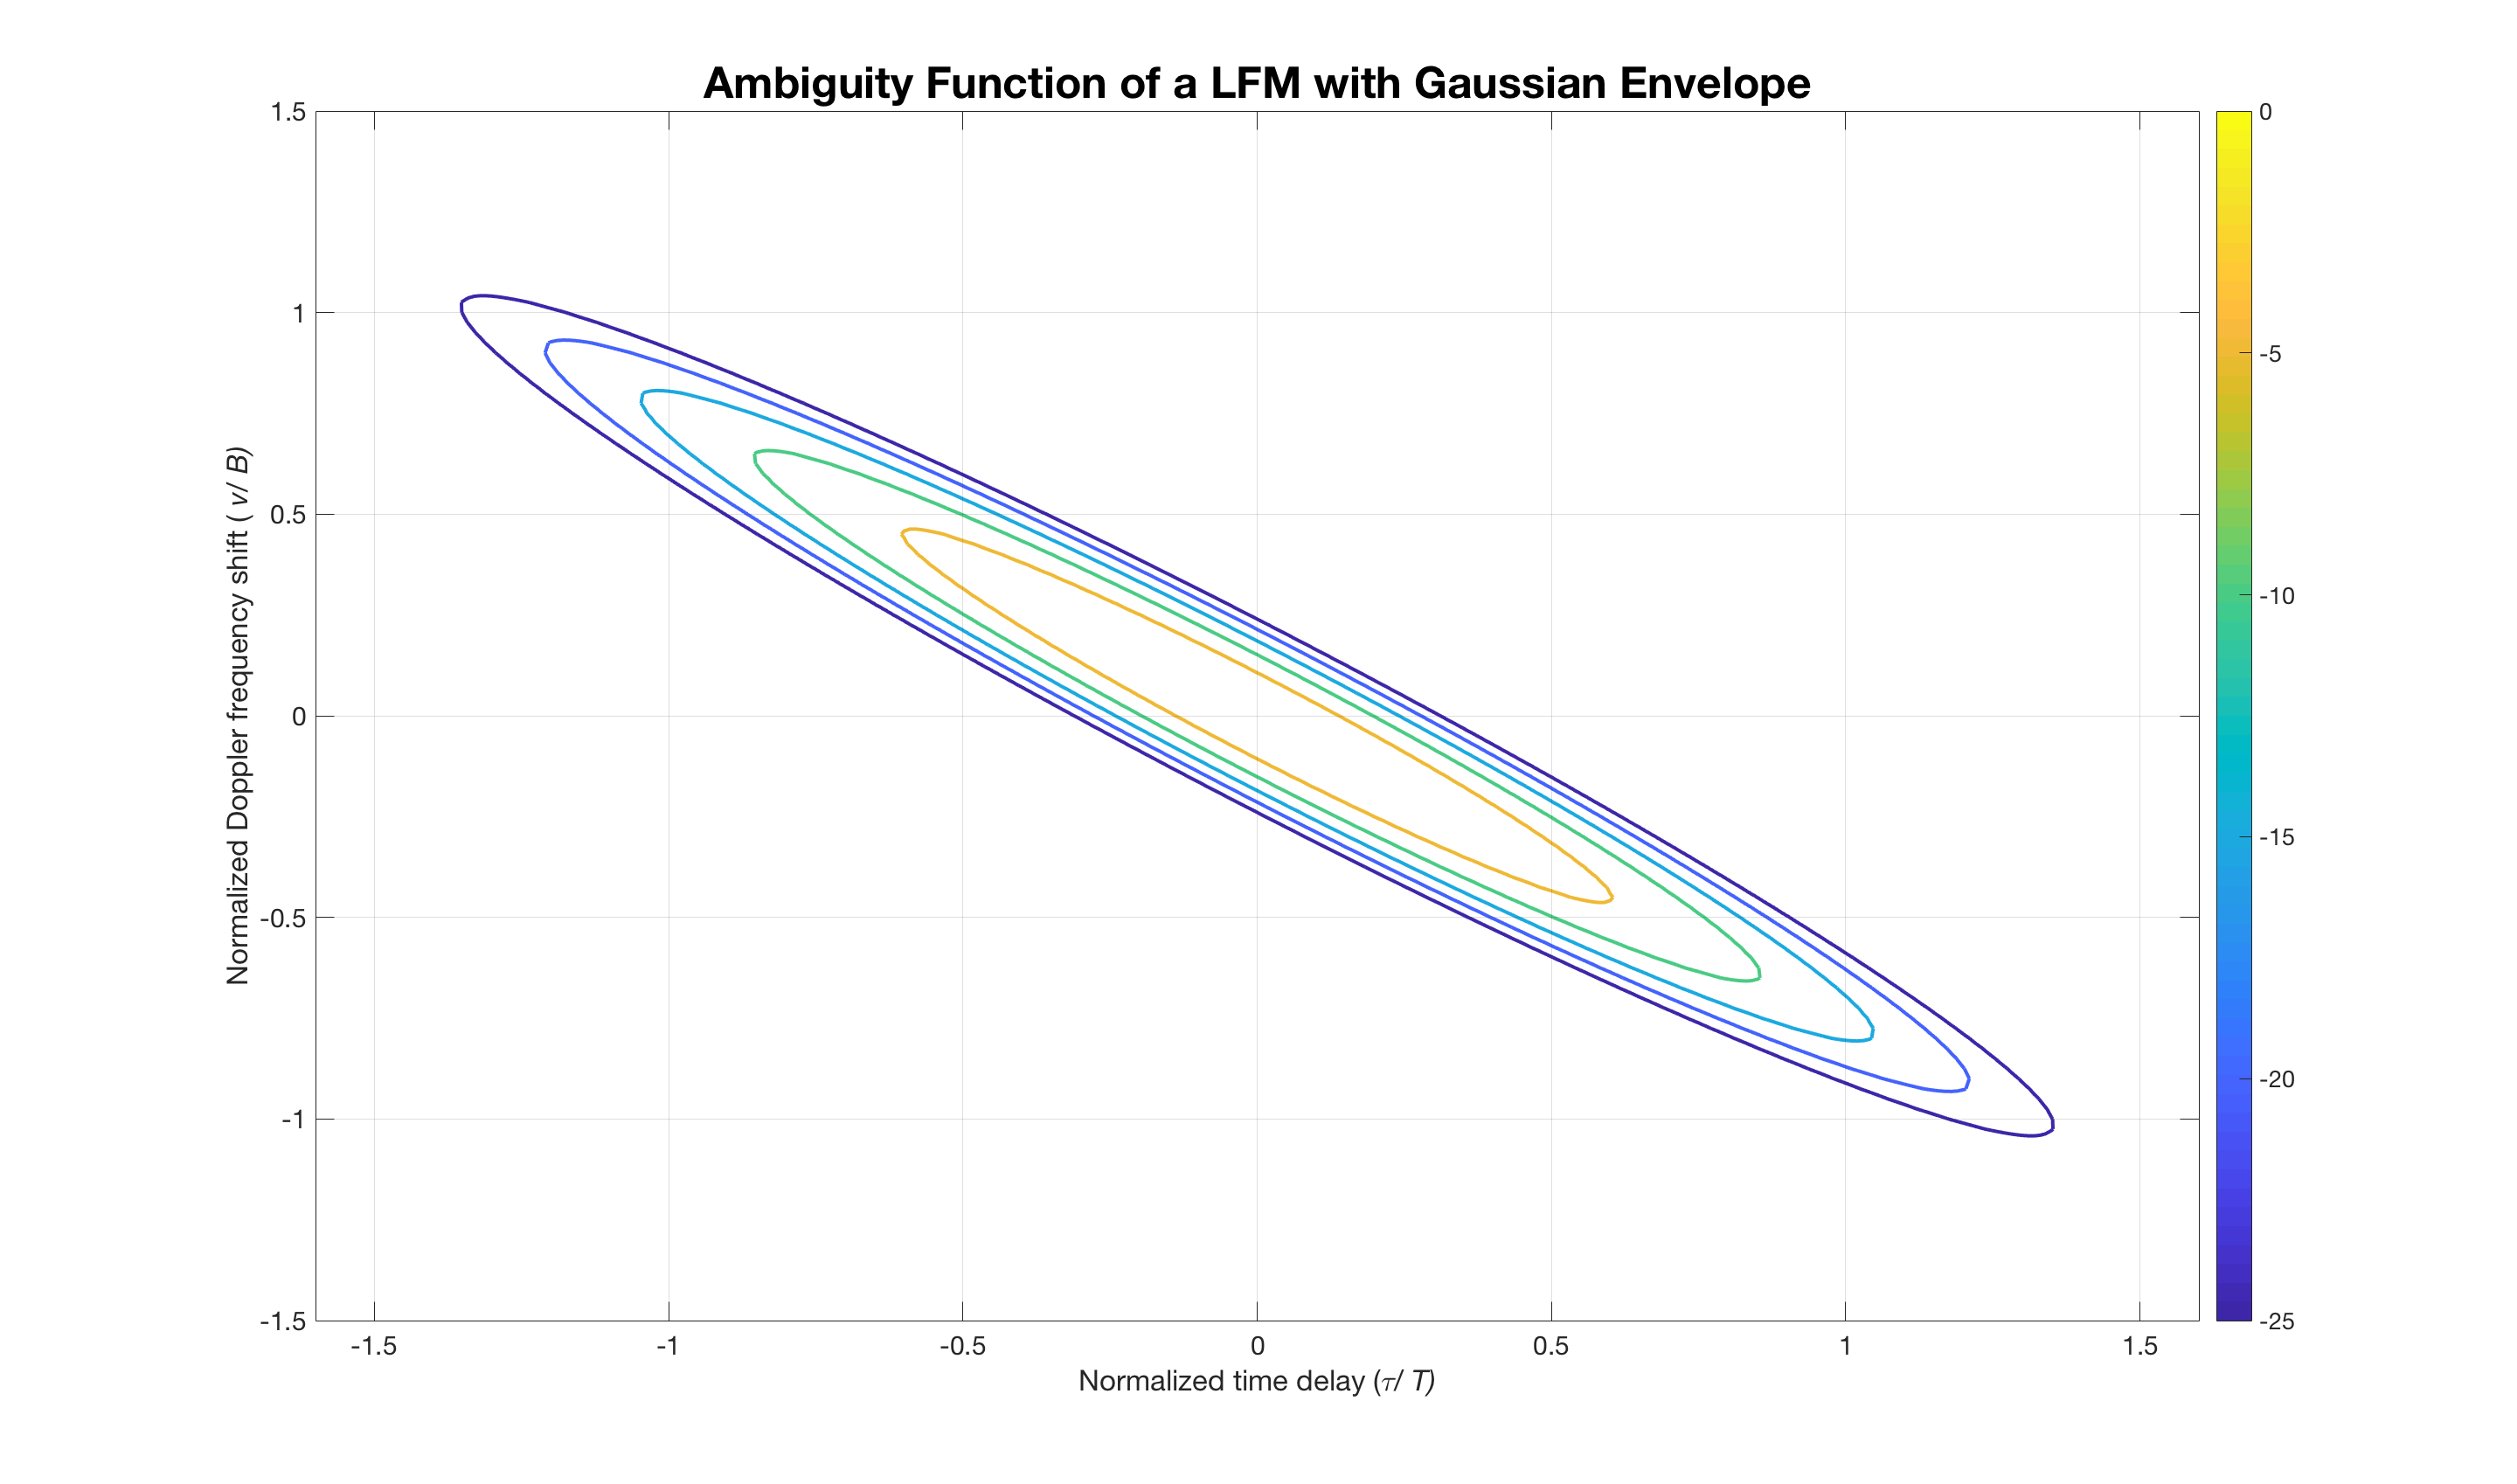
\includegraphics[scale=0.18]{usp8_6.png}}
\caption{ The ambiguity function of a Linear Frequency Modulated (LFM) pulse with Gaussian envelope }
\end{figure}

